\documentclass[a4paper]{report}
\usepackage[utf8]{inputenc}
\usepackage{epsfig}
\usepackage{graphicx}
\usepackage{amsmath}
\usepackage{amsthm}

\newtheorem{example}{Example}

\begin{document}

\begin{center}
    \begin{figure}[h!]
        \centerline{
\psfig{file=logo_unitn_black_center.eps,width=0.8\textwidth}}
    \end{figure}
    \vspace{2 cm}
    \Huge\textsc{Advanced Computing Architectures\\}
    \vspace{1 cm}
    \large{Passerone Roberto\\}
    \vspace{2 cm}
    
    \noindent\rule{12cm}{0.4pt} \\
        \medskip
        \textbf{Contributions are more than welcome} \medskip
        
        \small{If you spot any kind of typo or error, or if you wish to add material, don't hesitate to create a Pull Request or get in touch with us at \texttt{https://github.com/AlexSartori/AdvancedComputingArchitectures}.}
        \bigskip
    \noindent\rule{12cm}{0.4pt}
    
    \vspace{3 cm}
    \large{Notes curated by:\\Sartori Alessandro and Zanella Davide}
\end{center}

\clearpage

\tableofcontents

\chapter{Fundamentals of Computer Design}

\section{Power Consumption Evaluation}
In CMOS technology, power consumption is absorbed passively and actively. In the former case, power absorption is a symptom of inevitable current leakages between transistors' junctions, while in the latter case, current is drawn by logic gates when charging and discharging during operation and switching which, as a matter of fact, also causes transient short circuits, i.e. the control signal has finite slope and the N-MOS and P-MOS transistors won't switch perfectly in sync. 

\begin{figure}[htbp]
    \centering
    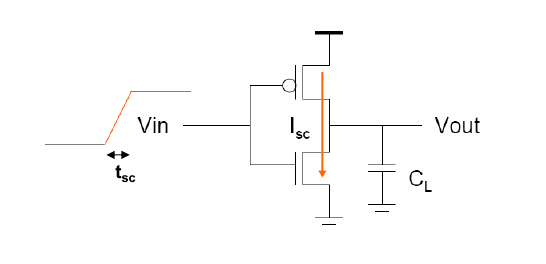
\includegraphics[width=0.7\textwidth]{images/logic_gate_1}
    \caption{Representation of a Logic Gate during a transient short-circuit: both transistors are conducting, creating a direct path to ground. $C_L$ is a parasitic capacitance responsible for most of the active energy consumption.}
    \label{fig:my_label}
\end{figure}

Active (or Dynamic) power consumption of a transition ($E_t$) is calculated by multiplying the energy necessary to switch state times the probability of this event (dependent for instance on the architecture). Power, being energy over time, equals energy times clock frequency.
\begin{align*}
E_t &= C_L \cdot V_{DD}^2 \cdot P_{0 \rightarrow 1} \\
\textrm{Power} &= C_L \cdot V_{DD}^2 \cdot P_{0 \rightarrow 1} \cdot f_{0 \rightarrow 1} = E_t \cdot \textrm{Frequency}
\end{align*}

Additionally, one needs to account for the mentioned short-circuits, absorbing a current proportional to the rising time of the signal $t_{sc}$:
\begin{align*}
E_{sc} &= t_{SC} \cdot V_{DD} \cdot I_{peak} \cdot P_{0 \rightarrow 1} \\
\textrm{Power} &= t_{sc} \cdot V_{DD} \cdot I_{peak} \cdot P_{0 \rightarrow 1} \cdot f_{0 \rightarrow 1} = E_{sc} \cdot f_{0 \rightarrow 1}
\end{align*}

Overall, dissipated power is given by the combination of:
\begin{itemize}
    \item $E_t$, mainly dependent on parasitic capacitance, therefore on number of gates and transistor size
    \item $E_{sc}$, dependent on transistor technology, size, temperature, and signal slope
    \item $E_{leakage} = V_{DD} \cdot I_{leakage}$, increasing with higher temperatures and lower threshold voltages
    \item $\textrm{Frequency}$, dependent on performance
    \item $P_{0 \rightarrow 1}$, dependent on signal statistics
\end{itemize}

Therefore:
\begin{align*}
    \textrm{Power} =&\ C_L \cdot V_{DD}^2 \cdot P_{0 \rightarrow 1} \cdot f_{0 \rightarrow 1}\\
    &\ + t_{sc} \cdot V_{DD} \cdot I_{peak} \cdot P_{0 \rightarrow 1} \cdot f_{0 \rightarrow 1}\\
    &\ + V_{DD} \cdot I_{leakage}
\end{align*}


\section{Cost Estimation}
Costs tend to generally decrease due to a number of factors. Manufacturing yield $Y$ for example, increases even without improvements in the implementation technology, adding up to an increase in production volumes which result in more amortized manufacturing costs. Costs trends also decrease because of competition effects, requiring selling prices to be close to production ones.

Experimentally, the cost $C$ of an integrated circuit is given by:
$$C=\frac{C_{die} + C_{testing} + C_{packaging}}{Y}$$
\noindent where $C_{die}$ is the cost of manufacturing a die, $C_{testing}$ that of testing a die after cutting it from a wafer, and $C_{packaging}$ that of packaging and testing the working ones. Unlike these last two costs which solely depend on the complexity of the IC, $C_{die}$ depends on more factors:
$$C_{die}=\frac{C_{wafer}}{N_{die} \cdot Y_{die}}$$
Where $N_{die}$, in turn, equals the number of dies on a round wafer of diameter $D$, minus those close to edge:
$$N_{die}=\frac{\textrm{Area of wafer}}{\textrm{Area of die}} - \textrm{Chips near the edge} = \frac{\pi \cdot \frac{1}{4} D^2}{A_{die}} - \frac{\pi \cdot D}{\sqrt{2 \cdot A_{die}}}$$
And $Y_{die}$ is given by:
$$Y_{die}=Y_{wafer} \cdot \left(1 + \frac{N_{defects} \cdot A_{die}}{\alpha}\right)^{-\alpha}$$
\noindent with $N_{defects}$ being the number of defects per unit area of the wafer, and $\alpha$ an empirical value related to manufacturing complexity.
\newline

In conclusion, it can be inferred that a designer only has control on the strong dependence that $A_{die}$ has on costs, while all other parameters only depend on the manufacturing process.


\section{Performance Evaluation}
...

\section{Design of Computing Systems}
...



\chapter{Instruction Set Architectures}



\chapter{Pipelining}

The basic idea of Pipelining is to divide the elementary operations related to a single instruction into a sequence of smaller task that can be performed in parallel.

The goal is to balance the length of each pipeline stage. In this way the time taken per instruction (pipelined) when the pipeline is full is:

\textit{Time per instruction (unpipelined)} / \textit{Number of stages}

\textbf{Pipelining reduces the average CPI.}

\section{Ideal pipelining}

\[ t_s = t_o + T_i/ p \]

where \\
$t_o$ is the overhead latency of each stage;\\
p is the number of stages; \\
$T_i$ is the total latency of a single instruction;

The \textbf{CPI} is the number of clocks required (on average) to complete one instruction after the previous one has completed.

In a pipeline, the throughput of any instruction sequence (i.e., the number of completed instruction per unit of time) is \textbf{about p times larger} than in the unpipelined solution.
CPI is asymptotically equal to 1.
Average Instruction Execution Time $T_e = T_{CLK} * CPI$

\section{Pipeline in a RISC CPU (MIPS)}
\paragraph{MIPS features}
\begin{itemize}
    \item 32 64-bit general purpose register (GPR), named R0, R1, ..., R31. (R0 = 0)
    \item 32 floating-point registers (FPR), named F0, F1, ..., F31.
    \item Data types: 8-bit bytes, 16-bit half words, 32-bit words, 64-bit double words.
    \item Addressing modes:
    \begin{itemize}
        \item Immediate: ADD R4, \#3
        \item Displacement: LD R4, 100(R1)
        \item Register indirect: LD R4, 0(R1)
        \item Absolute addressing: LD R4, 2536(R0)
    \end{itemize}
    \item Load/store architecture
\end{itemize}

\subsection{Instruction Execution stages}
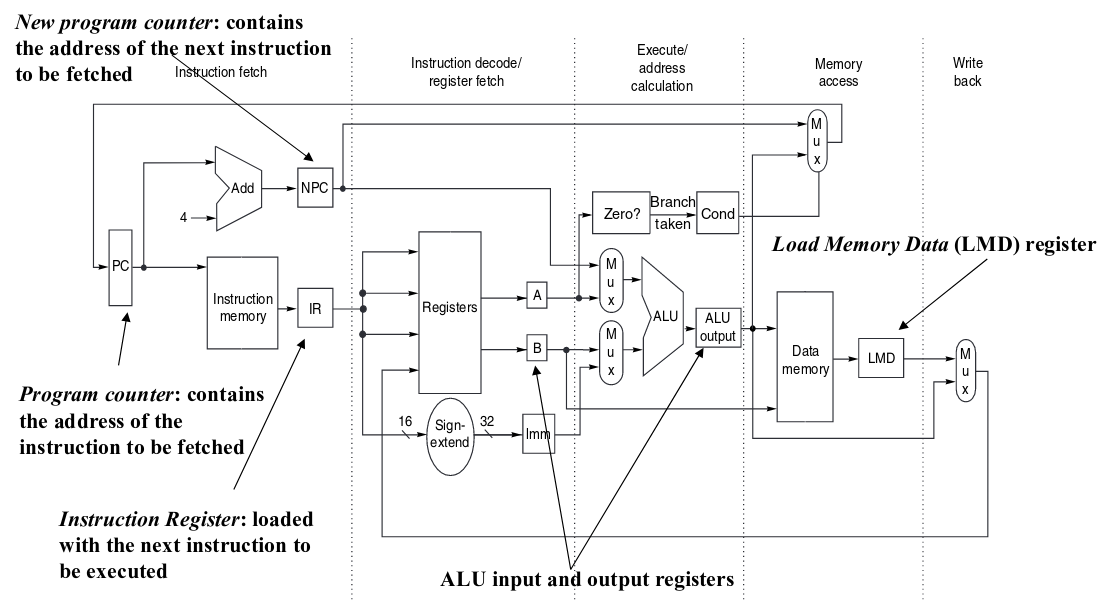
\includegraphics[width=\textwidth]{images/mips_scheme.png}

Stages:
 \begin{itemize}
    \item \textit{Instruction fetch stage (IF)}:\\ Send the program counter (PC) to memory and fetch the current instruction from memory or I-cache. Update the PC to next sequential value (e.g. by adding 4 if an instruction is 4 byte long)
    \item \textit{Instruction Decode/ register fetch stage (ID)}:\\decode the instruction and perform simultaneous operand reading. Instruction decode and operand reading can be done in parallel because RISC instructions are fixed-field encoded. \\
    • In case of register operands read the source registers values from the register file\\
    • In case of immediate operands, sign-extend the offset field of the instruction
    \item \textit{Execution/effective address stage (EX)}:\\
    The ALU operates on the operands prepared in the previous cycle, performing different operations depending on the instruction type.\\
    • Load/store instructions: The ALU adds the base register and the offset to form the effective address. \\
    • Register-Register ALU instructions: The ALU performs the operation specified in the ALU opcode on the values read from the register file \\
    • Register-Immediate ALU instructions:The ALU performs the operation specified by the ALU opcode on the value read from the specified register and the sign-extended immediate \\
    • Branch instructions: The ALU adds the next instruction value to the extended value of the address (multiplied by 4) to calculate the branch target address (BTA).
    In conditional branches the value of the condition register is compared with the reference value (i.e., 0) and stored into a special register.
    \item \textit{Memory access stage(MEM)}:\\
    – Load instructions: The memory performs a read using the effective address computed in the previous cycle using A and Imm and saved in ALU output\\
    – Store instructions: The memory performs a write using the effective address computed in the previous cycle using A and Imm and saved in ALU output, while the value comes from the other register, saved in B\\
    – Branch instructions: in branches, the PC is replaced with the BTA (saved in ALU output) according to the outcome of the comparison with zero, saved in Cond
    \item \textit{Write-back stage(WB)}:\\
    –Loads and ALU instructions: Write the result into the register file, whether it comes from the memory system (for a load) or from the ALU (for an ALU instruction)
\end{itemize}

It is important to \textbf{perform approximately the same amount of work in each stage}. In fact, the clock cycle of the processor depends on latency of the stage with the worst-case delay.

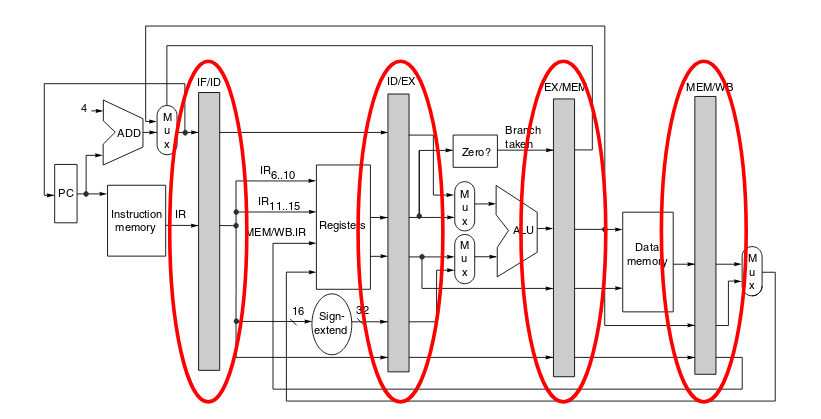
\includegraphics[width=\textwidth]{images/mips_pipeline.png}

Instructions are fetched and initiated at every clock cycle filling all the stages. In this way the CPU will be perfectly busy. For this, the following basic modifications have to be applied:
\begin{itemize}
\item Insert homogeneous registers or latches between stages (IF/ID, ID/EX, EX/MEM, MEM/WB) thus replacing (i.e. including) temporary registers
\item Propagate the control signals generated by the CU as well as the status bits of each instruction within the same pipeline registers
\item Anticipate the PC contents update operation to the IF stage (instead of running it in the MEM stage) to avoid fetch latencies
\end{itemize}

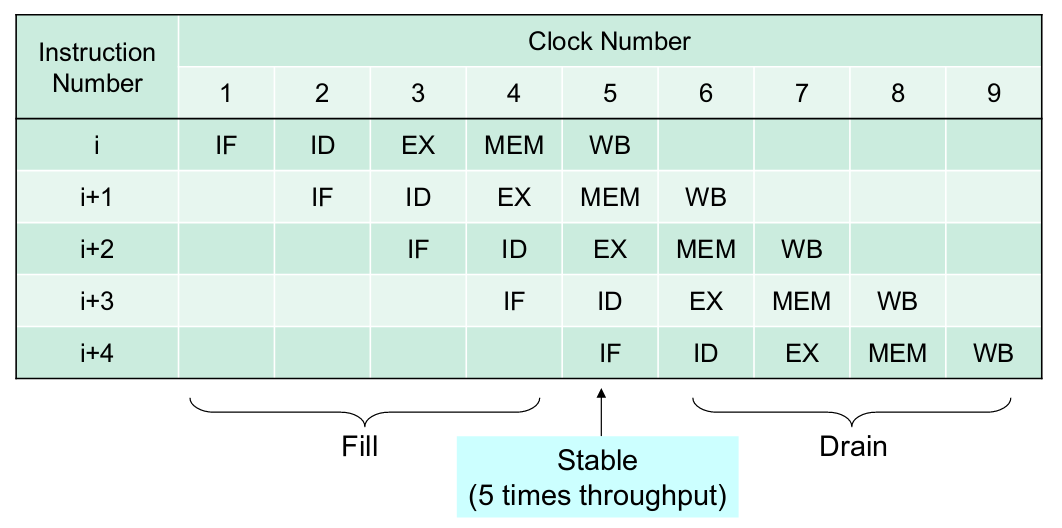
\includegraphics[width=\textwidth]{images/mips_pipeline_stages.png}

Why isn't the speed-up = 5?
The unpipelined version skips certain stages when not needed and the pipelined version has a 20\% clock overhead.

\section{Hazards}
The presence of several instructions simultaneously active into the pipeline may lead to various type of dependencies which turn into hazards. Hazards reduce the performance from the ideal speedup by forcing the pipeline to \textbf{stall}, i.e., to delay subsequent instructions until the source of the hazard is solved. Hazards can be solved using \textit{hardware techniques}, \textit{software techniques} or a combination of both.

\subsection{Structural hazard}
Arise from resource conflicts when the hardware can not support all possible combinations of instructions at the same time.

In a pipelined processor, the overlapped execution of instructions requires pipelining of functional units and duplication of resources. If some combination of instruction requires to use the same resource a structural hazard arise.

To avoid structural hazards (which would lead to incorrect results), the pipeline is stalled -> 1  or more “empty”cycles or bubbles are inserted in the pipeline.

\textbf{Stalls result in a reduction of instruction throughput.}

Other solutions:
\begin{itemize}
    \item Hardware:\\
    Resource splitting/replication but it's expensive!
    \item Software:\\
    Instructions requesting the same resource are located at proper distance from each other. For instance, two conflicting instructions could be delayed by the compiler. It's effective but compiler design could be cumbersome!
\end{itemize}

\paragraph{Impact of hazards on CPI}
Say the probability of a stall is 20\%: 1 stall every 5 instructions

$CPI = \frac{\#clocks}{\#instr} = \frac{IC + (\frac{IC}{5} - 1)}{IC} = 1 + \frac{1}{5} - \frac{1}{IC}$

\subsection{Data hazard}
Data hazards are related to \textbf{data dependencies}, i.e., sequential constraints imposed by the data flow of the program.
Two different instructions are data dependent if they have a common register or memory location; unless the operand is for both a \textit{source operand}.

Data dependencies can occur in:
\begin{itemize}
    \item \textbf{Straight-line code}: between subsequent instructions during the execution of a program segment
    \item \textbf{Loops}: between instructions belonging to different iterations of the loop (also called \textit{recurrences} or \textit{inter-iteration dependences})\\
Example: first-order linear recurrences: e.g.: X(i) = A(i) * X(i-1) + B(i)
\end{itemize}

Three kinds of data dependences:
\begin{itemize}
    \item \textbf{Read after Write (RAW)} also called flow or true dependence\\
    A read uses the value written by a write instruction.\\
    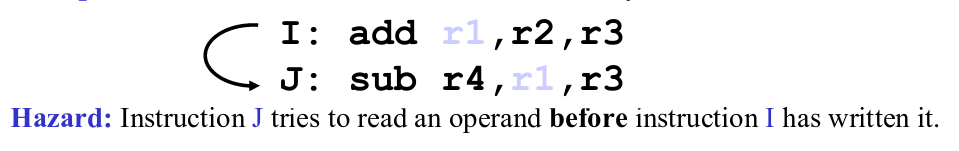
\includegraphics[width=\textwidth]{images/RAW_scheme.png}
    
    \item \textbf{Write after Read (WAR)} also called anti dependence\\
    The destination of an instruction is a source operand of a previous instruction.\\
    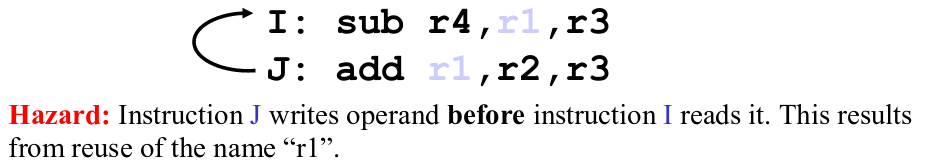
\includegraphics[width=\textwidth]{images/WAR_scheme.png}
    
    \item \textbf{Write after Write (WAW)} also called output dependence\\
    Two instructions have the same destination operand.\\
    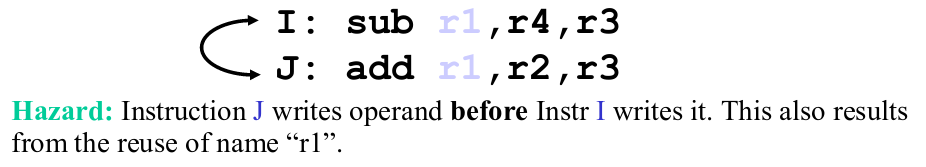
\includegraphics[width=\textwidth]{images/WAW_scheme.png}
\end{itemize}

\paragraph{Solutions to data hazards}
\begin{itemize}
    \item WAR, WAW are \textbf{false dependences}: 
    they can be solved through renaming (during compilation or by means of specialized hardware)\\
    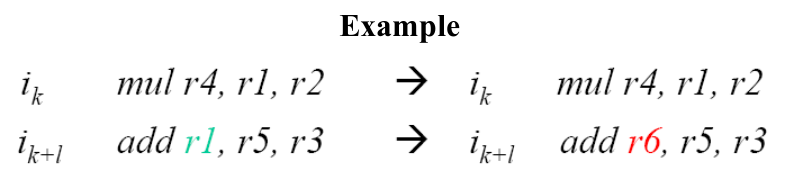
\includegraphics[width=\textwidth]{images/renaming_solution_data_hazard.png}
    
    \item RAWs are \textbf{true dependences}
\end{itemize}

One RAW hazard example on a 5-stage pipeline:\\
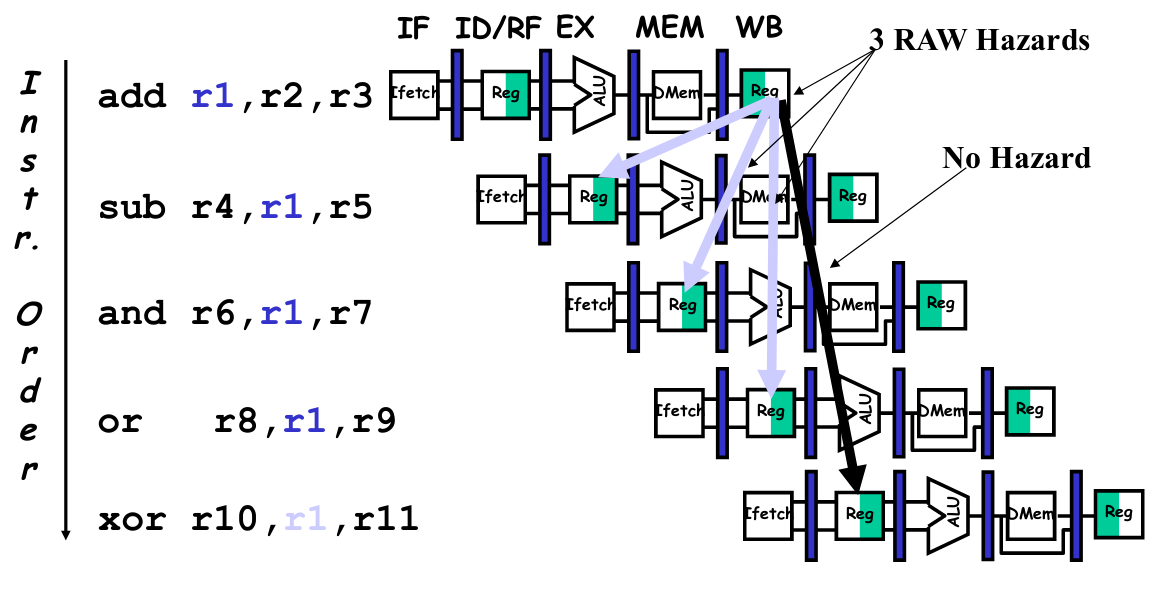
\includegraphics[width=\textwidth]{images/RAW_hazard_example.png}

\paragraph{Software solutions}
\begin{itemize}
    \item \textit{Code moving}:\\
    If possible, the compiler inserts as many non-dependent instructions as necessary (3 instructions in the case considered) between define and first use of a variable.\\
    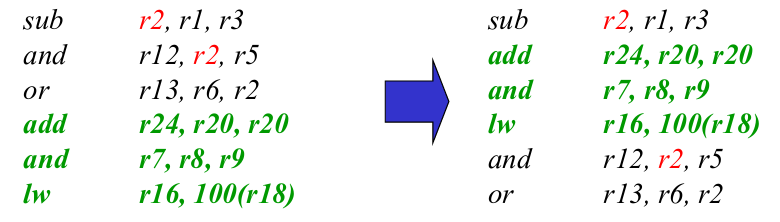
\includegraphics[width=\textwidth]{images/data_hazard_sol1.png}
    
    \item \textit{Nop stuffing}:\\
    The compiler inserts as many nop as are the required cycles between define and first use; So do not perform any active computation.\\
    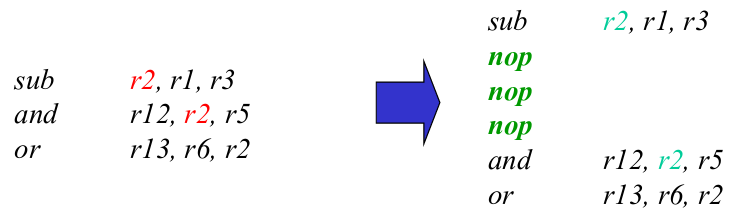
\includegraphics[width=\textwidth]{images/data_hazard_sol2.png}
\end{itemize}

\paragraph{Hardware solutions}
The CU of the pipeline:
\begin{enumerate}
    \item Check (in the ID stage) whether one of the source register $r_{s1}$ and $r_{s2}$ of the considered instruction $I_{k+1}$ coincides with the destination register $r_d$ of some previous incomplete instruction. 6 comparisons are required:\\
    IF/ID.IR($r_{s1}$) == ID/EX.IR($r_d$) \|  IF/ID.IR($r_{s2}$) == ID/EX.IR($r_d$)\\
    IF/ID.IR($r_{s1}$) == EX/MEM.IR($r_d$) \|  IF/ID.IR($r_{s2}$) == EX/MEM.IR($r_d$)\\
    IF/ID.IR($r_{s1}$) == MEM/WB.IR($r_d$) \|  IF/ID.IR($r_{s2}$) == MEM/WB.IR($r_d$)
    
    \item If a hazard is detected, the CU stalls the conflicting instruction $I_{k+1}$ in the ID stage until the instruction $I_k$ has completed its flow (pipeline interlock). Same as a nop but with less instruction memory space.
\end{enumerate}
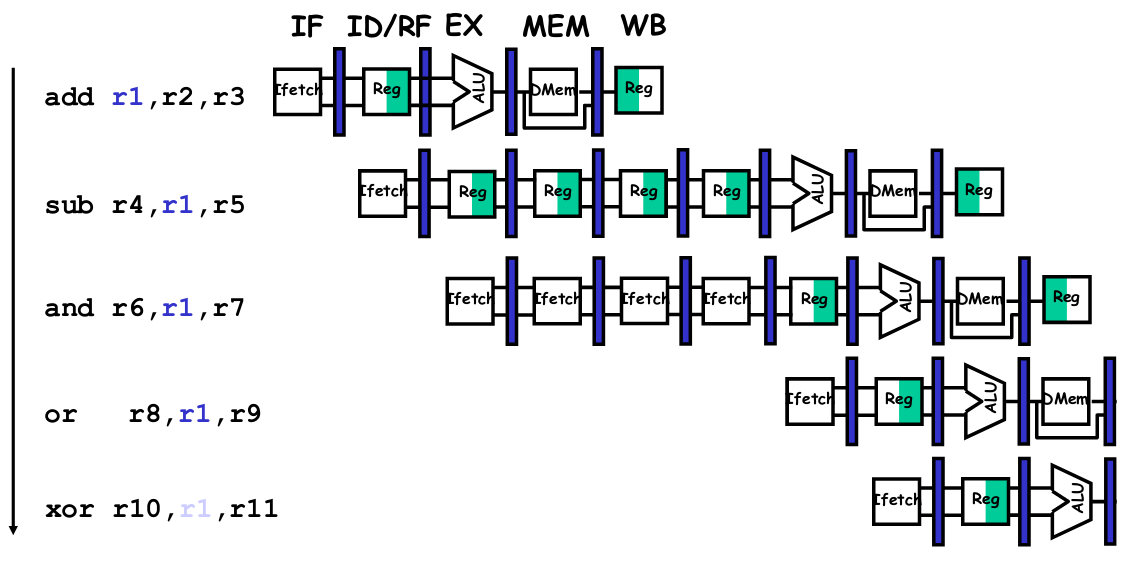
\includegraphics[width=\textwidth]{images/pipeline_CU_scheme.png}

\paragraph{Forwarding}
We can use forwarding to reduce the stall penalty. Briefly in some cases instead of waiting that the information will be written in the registers we can simply forward them from a inter-stage pipeline register to another one.

Thus we can implement forwarding control by multiple comparisons between EX/MEM.IR(rd) and MEM/WB.IR(rd) with ID/EX.IR(rs) and EX/MEM.IR(rs). Increasing HW complexity due to comparators and MUX enlargement.

Not all RAW hazard can be handled by forwarding. This happens when certain data is required at ALU inputs before it is ready. In this case forwarding reduces stall penalty, but it can not prevent some “bubbles”.

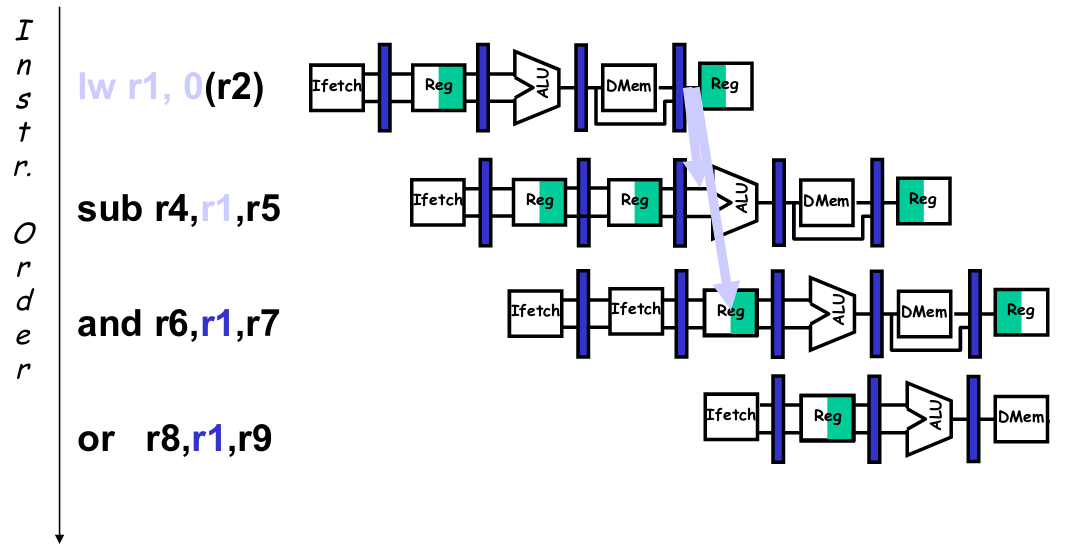
\includegraphics[width=\textwidth]{images/pipeline_scheme_forwarding.png}

\subsection{Control hazard}
Control dependences are sequential constraints due to the control flow of the program.
All branch instructions (e.g. jumps, procedure calls and returns, traps, interrupt) create control dependences.

If a branch changes the PC, it is referred to as a \textbf{taken branch}; if it falls through, it is not taken, or \textbf{untaken}.

\textit{Control hazards} are related to the risk of fetching into the pipeline the wrong instructions following a conditional branch before knowing if the branch has to be taken or not.
For example when we have a beq followed by some other instructions, without any control the following instructions will be fetched before the beq instruction enters in the MEM stage. There is a control hazard.

\paragraph{Solutions}
\begin{enumerate}
    \item \textit{Freezeor flush the pipeline}:\\
    Hold or delete any instruction after the branch until the BTA is known
    \item \textit{Predict branch as not taken}:\\
    As PC+4 is already calculated, the hardware continues to fetch instructions in sequence as if the branch were not executed. If the branch is actually taken, wrongly fetched instructions have to be “flushed” (i.e., turned into nops)
    \item \textit{Predict Branch as Taken}:\\
    As soon as the branch is decoded and the BTA is calculated, we begin fetching instructions from BTA. If the branch was not to be taken, wrongly fetched instructions are “flushed” (like in solution 2).This solution is meaningful only if the BTA is known before branch outcome.
    \item \textit{Branch hoisting (delay slots)}:\\
    The compiler moves 3 independent instructions that have to be executed in any case immediately after the branch instruction into the so-called branch delay slots. When such instructions are complete the branch outcome is known and no stalls are required.
\end{enumerate}

To reduce the control hazard time penalty, we can shift both the decision about taken or not taken and the BTA calculation in the ID stage. This requires an additional adder, but it decreases the possible stalls from 3 to 1.
This is not a general rule. In deeply pipelined processors, the control hazard penalties could be very large in terms of wasted clock cycles and can not be solved so easily.

\subsection{Performance of pipelines with stalls}
$Speedup = \frac{CPI_{unpipelined}}{CPI_{pipelined}} * \frac{Tclk_{unpipelined}}{Tclk_{pipelined}}$
\\
$CPI_{pipelined} = Ideal CPI + N_{stalls} = 1 + N_{stalls}$

If we ignore the pipeline overhead time we have that: $Tclk_unpelined = Tclk_pipelined$\\
If all instructions take the same number of cycles: $CPI_{unpipelined} = pipeline-depth$

\section{Exception}
The term exceptions cover all the possible exceptional situations whereby the normal execution order of instructions is changed.

Many differences exist between various CPUs.

\paragraph{Some sources of exception}
\begin{enumerate}
    \item Conditions arising from instruction execution (e.g., overflow, FP anomaly)
    \item External interrupts (e.g., I/O device request)
    \item System calls (traps)
    \item Memory-related exceptions (e.g., cache misses, page fault, memory protection violation, misaligned memory access)
    \item Undefined Opcode6.Hardware malfunctions and power failures
\end{enumerate}

\paragraph{Some features}
\begin{itemize}
    \item Synchronous vs. Asynchronous
    \item User requested vs. coerced
    \item User maskable vs. unmaskable
    \item Within vs. between instructions
    \item Resume vs. terminate
\end{itemize}

\paragraph{Exception handling}
\begin{enumerate}
    \item Exception is associated with the only instruction presently being executed
    \item Exceptions are managed by appropriate routines (e.g., Exception Service Routine or ESR)
    \item When an exception is detected, the CU looks into a vector table. Each row of this table contains the memory address of the corresponding ESR
    \item The ESR saves the PC of the excepting instruction, runs the instruction to handle the corresponding exception and finally returns to the original program if the exception requires resuming 
\end{enumerate}

In pipelined CPUs, the situation is much more involved because concurrent instructions are active in the pipeline. Two main problems:
\begin{enumerate}
    \item Recognizing the exception (i.e., associating it with the correct instruction)
    \item Saving the correct machine state
\end{enumerate}

\paragraph{Some exception examples in a pipeline}

\begin{itemize}
    \item \textit{Exceptions arising from instruction execution (e.g. overflow)}: usually raised during stage EX(i.e., within an instruction). They are also coerced, generally user-maskable and they require a resume. 
    \item \textit{External (I/O) interrupts}: Asynchronous, coerced exceptions requiring a resume. The ISR are usually served when the interrupted instruction is in the WB stage(i.e., between subsequent instructions).
    \item \textit{Cache miss}: actually, only data cache miss are considered exceptions (instruction cache misses are directly managed by hardware, which stalls the CPU before IF phase). These exceptions (like page faults) are detected in MEM stage, are coerced, synchronous and non-maskable.
    \item \textit{Non-existing OP code}: may be due to a compiler error, to a memory fault but also, in CPUs belonging to “families”, to instructions invoking functional units not present in the particular device used. This exception is raised in the ID stage;it is synchronous, coerced, non-maskable and leads to program termination.
\end{itemize}

\section{Advanced pipelining}
\subsection{Superpipelining}
A superpipelined processor has a pipeline where each logical step (IF, ID, EX, MEM, WB) is subdivided into simpler multiple pipeline stages. So smaller $T_{CLK}$.

Reduction of stage complexity is limited by four factors:
\begin{enumerate}
    \item \textit{Imbalance problems}:\\
    Imbalance between stages reduces performance because the clock period can not be shorter than the time needed for the slowest pipeline stage
    \item \textit{Pipeline overhead time}:\\
    It results from the combination of two contributions:
    \begin{itemize}
        \item Pipeline register delay: this is due to setup and propagation time through the register. This is constant and related to technology 
        \item Clock skew: worst-case delay between active clock signal edges in two points of a digital system (e.g., between any two pipeline registers)
    \end{itemize}
    The sum of these two contributions represents lower bound to clock cycle.
    \item \textit{Growing data dependences}:\\
    This leads to a higher number of bubbles in a deeper pipeline–performance loss due to data hazards increases
    \item \textit{Longer control hazards}:\\
    imply slower branches in case of wrong predictions
\end{enumerate}

Summing up: cycle time is shorter but the number of cycles required by a given program becomes larger.

Certain operations, such as floating point, may require multiple cycles to complete so it's impractical to have them complete in one cycle.
The EX stage will be repeated as many times as necessary.

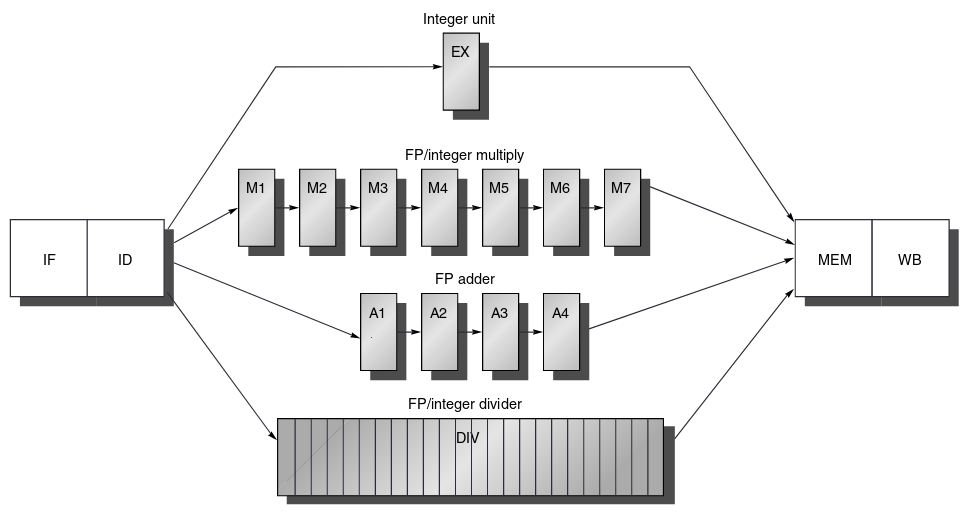
\includegraphics[width=\textwidth]{images/superpipeline.png}

\paragraph{Problems}
\begin{itemize}
    \item Instructions may complete in a different order than they were issued
    \item WAW hazards are now possible, since instructions no longer reach WB in order
    \item WAR are still not possible, since registers are still read in ID, and instructions go through ID in order
    \item Stalls due to RAW will be more frequent, since instructions have longer latency. Instructions stalls for long periods awaiting the results from the floating point operations.
    \item Structural hazard: Instructions reach MEM and WB simultaneously!
\end{itemize}

\subsection{Superscalar}
Superscalar architecture is a single processor that can execute several scalar operations in parallel.
\begin{itemize}
    \item Using different dedicated pipelines, implemented on the basis of the classes of instructions that are more frequently used on a given architecture.
    \item Using multiple identical pipelines, i.e. multiple copies of a given physical pipeline.
\end{itemize}


\chapter{Memory organization}

Larger memories are slower than smaller memories.
Fast memories are much more expensive than slow memories.

So instead of using a single large memory, modern systems use a hierarchy. 
Characterized by different technology, cost, dimensions and access mechanisms. The programmer sees an unique large memory space. The CPU sees a fast memory at acceptable cost.

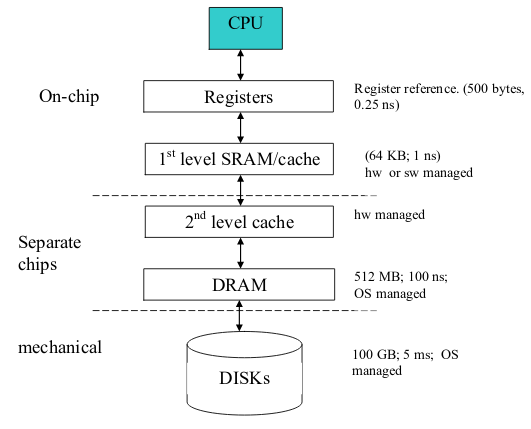
\includegraphics[width=.7\textwidth]{images/memory_hierarchy.png}
Hierarchies work well because memory access follows the principle of locality.

\paragraph{Locality}
\begin{itemize}
    \item \textbf{Temporal locality}:\\
    when a memory entry is referenced, with high probability it will be referenced again within a short time.
    
    \item \textbf{Spatial locality}:\\
    whenever a memory entry is referenced, with high probability reference will be made shortly to neighboring items.
\end{itemize}

\paragraph{Registers}
Registers are usually “exposed” to the programmer. Alternatively, the compiler allocates variables to registers.
Registers are usually placed into a regular register file. A register file consists of multiple read/write ports to allow parallel, simultaneous data accesses.
Typically, at least 2 read and 1 write ports are required to access operands of a single instruction.

Unfortunately, the size of the register file grows with the square of the number of ports so an excessive number of ports slows down the processors.

This quadratic increase in chip area is mostly due to the new additional input and output lines:\\
• Routing problems\\
• Internal bit cell loading increases -> larger power consumption\\
• Linear increment in delay with the number of ports

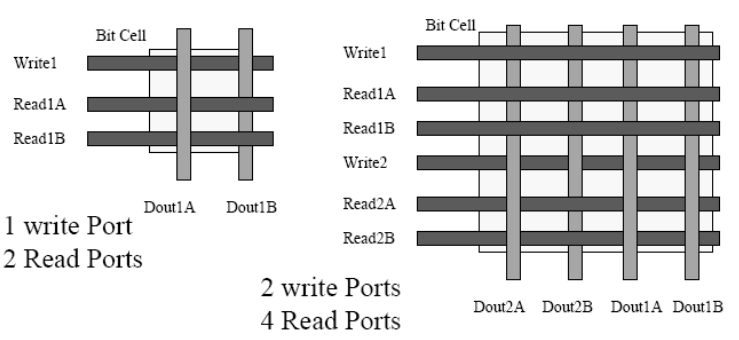
\includegraphics[width=.7\textwidth]{images/memory_bit_cells.png}

It is not profitable to have a register file with more than 15-20 ports: 12 is actually the best tradeoff when number of FU is larger than 4

\paragraph{The usual SRAM}
\begin{itemize}
    \item It is “exposed” to programmer and compiler
    \item Data transfers from/to memory are performed by \textbf{software}
    \item It is mostly used in low-end or specialized embedded processors where worst-case latency to recover data and power are the main issues
\end{itemize}

\paragraph{Cache}
\begin{itemize}
    \item Usually it is “transparent” to programmer and compiler
    \item Transfers from/to lower-level memories are performed by \textbf{hardware}
    \item It is mostly used in high-end processors where the power is less critical and average performance should be maximized
\end{itemize}

\paragraph{Scratch Pad}
It's a low power consumption solution.
The scratch pad is a buffer of memory (no cache) where most frequently used program functions instructions and data are allocated.
This approach requires a preliminary “profiling”to decide what instructions have to be placed into the scratch pad.
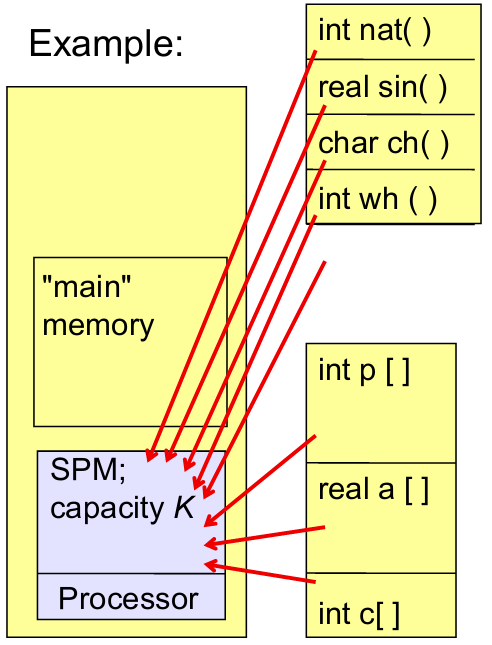
\includegraphics[width=.5\textwidth]{images/memory_scratch_pad.png}
Allocation usually performed statically at compile time (no HW support).
This kind of solution is very used in embedded systems because the program is usually fixed and it is a reasonable tradeoff between performance and power consumption.

\paragraph{Cache}
A cache is a special kind of memory based on SRAM cells which is used to store the data having the maximum probability to be used.
Cache can be either unified (i.e., simultaneously instruction-and data-cache) or split into I-cache and D-cache.

Definitions:
\begin{itemize}
    \item \textbf{Hit}: the item requested by the CPU is present in cache
    \item \textbf{Miss}: the item requested by the CPU is not present in cache
    \item \textbf{Hit rate}: fraction of memory accesses rewarded by hit
    \item \textbf{Miss rate}: fraction of memory accesses resulting in a miss (miss rate = 1 -hit rate)
    \item \textbf{Hit time}: access time (or clock cycles) to cache in the case of success (includes time to determine whether access is met by hit or miss)
    \item \textbf{Miss penalty}: time (or clock cycles) required to substitute a block of data in cache with another block from the lower-level storage
    \item \textbf{Miss time}: miss penalty + hit time, time required to obtain requested data in the case of miss
\end{itemize}

Cache performance is given in terms of average memory access time (AMAT)

$AMAT = hit-time + miss-rate * miss-penalty$\\

Cache performance affects CPU time

$CPU_{time} = IC * (CPI_{execution} + \frac{MEM_{accesses}}{IC} * miss-rate * miss-penalty) * T_{CLK}$

\paragraph{How cache works}
A cache is made of a number of \textbf{blocks} that contain \textbf{words} from memory.
The size of a block is a power of 2, to simplify addressing (e.g., a block is made of 32 words).
When a word is needed, its entire block is loaded from memory and placed somewhere in the cache.
Blocks that are next to each other in memory are not necessarily stored next to each other in the cache, and vice-versa.

The cache needs to store a block along with its actual address in memory.
The required address is compared to the address of all the blocks in the cache to find a match.
If found, it is a hit, otherwise it is a miss.

\paragraph{Problems in cache design}
\begin{itemize}
    \item \textbf{Placement problem}:\\
    Where to place a block transferred from lower to higher level
    \item \textbf{Search (or identification) problem}:\\
    how to determine whether the requested item is present or not
    \item \textbf{Substitution (or replacement) problem}:\\
    Which block present in the cache must be replaced by one in lower-level storage, in the case of a miss
    \item \textbf{Write strategy}:\\
    what happens when a write-to-memory instructions is executed?
\end{itemize}

\section{Direct-mapped cache}
Assume the cache is made of an array of $N_B$ blocks.
Let $B_{AR}$ be the address of the required block in RAM.

In a direct-mapped cache, the block can only be placed in the cache block at address $B_{AC}$:

$B_{AC} = B_{AR} mod N_B$

$B_{AC}$ is also called the index of the cache block.
If $N_B$ is a power of 2, then the index is equal to the $N_{AC} = log2(N_{B}$ least significant bits of $B_{AR}$.

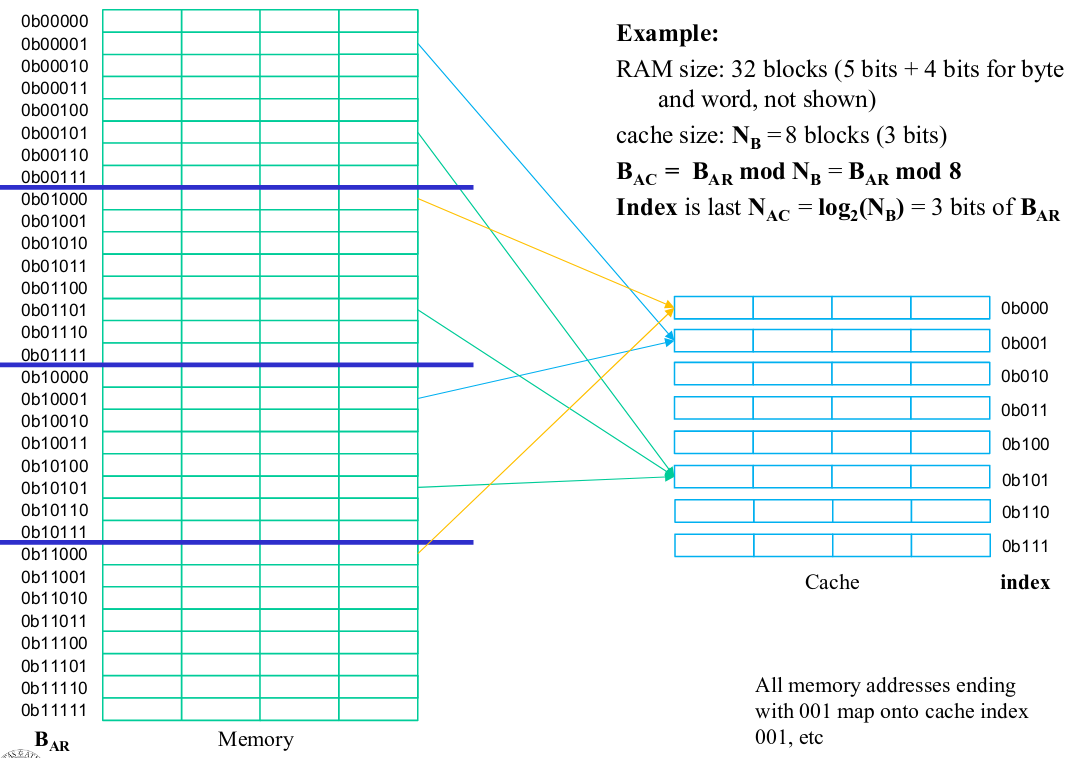
\includegraphics[width=\textwidth]{images/direct_mapped_cache.png}

\paragraph{Problems}
\begin{itemize}
    \item \textbf{Placement problem}:\\
    Trivial – the block from RAM can be mapped onto one cache block only
    \item \textbf{Search problem}:\\
    different memory blocks can be placed in the same cache block. How do we decide which location is mapped in the cache?\\
    \textbf{Solution}: each cache line must be provided with:
    \begin{itemize}
        \item A \textbf{tag field} containing the $N_{AR} - N_{AC}$ most significant bits of $B_{AR}$
        \item A \textbf{validity bit} - denotes whether block contains meaningful (valid) data.
    \end{itemize}
    \item \textbf{Replacement problem}:\\
    Trivial – the new block from RAM can be mapped onto one cache block only. Does not account for temporal locality! Block substituted may have been very recently used.
\end{itemize}

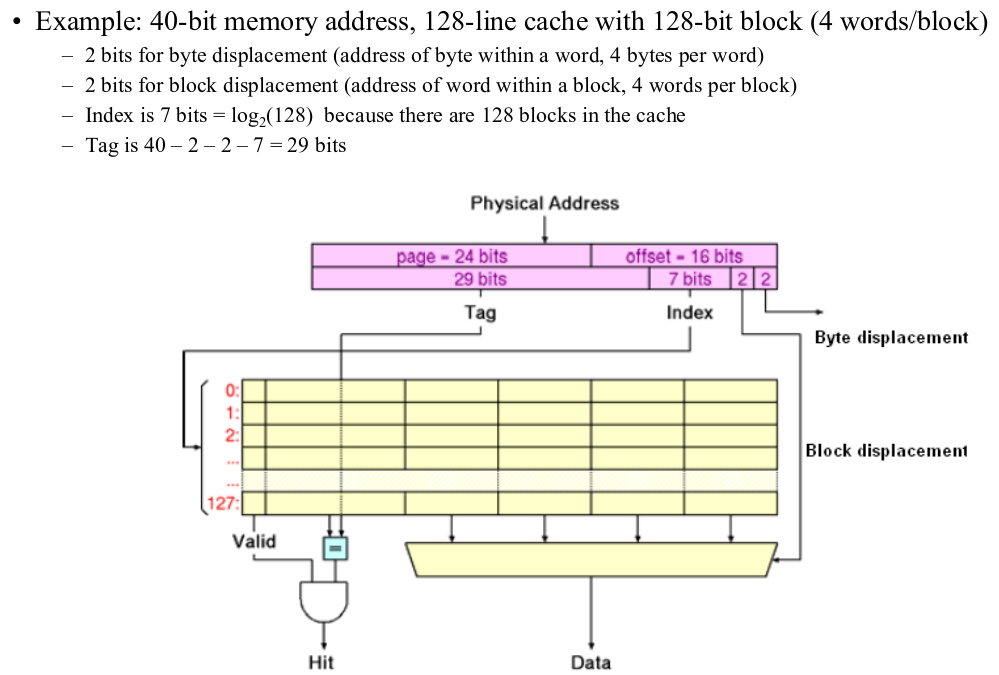
\includegraphics[width=\textwidth]{images/direct_mapped_cache_example.png}

\section{Fully associative cache}
In fully-associative cache every block of RAM can be mapped onto any block of cache (there is no constraint on Placement).
The search problem is tackled by running a parallel comparison of  the wanted address with all tags. So a large number of comparators is done and so it's very expensive in terms of area and power consumption.

The index is 0 bits and the tag is the complete address of the word minus the bits for block and byte displacements. 

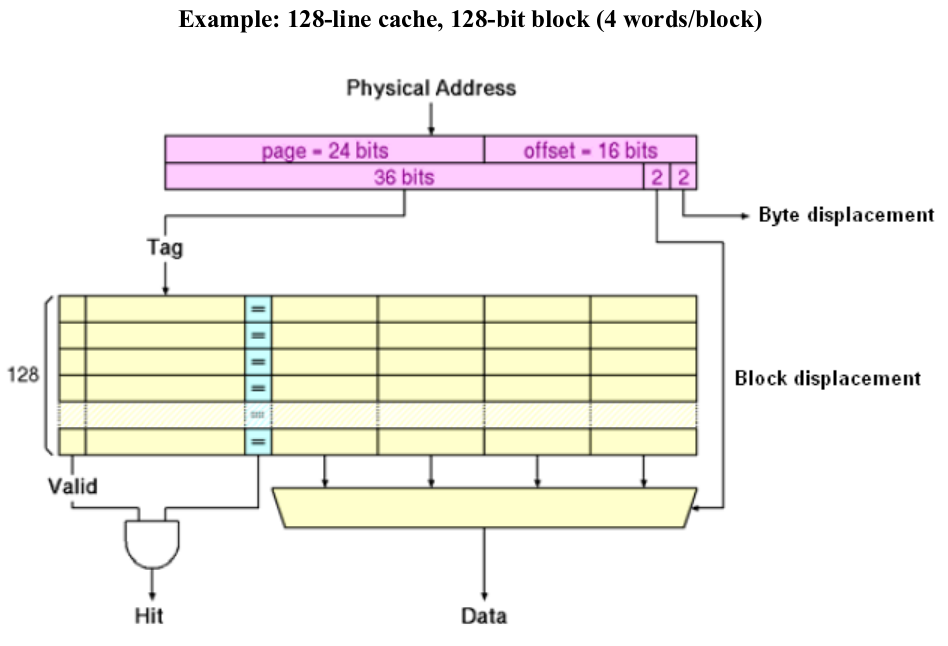
\includegraphics[width=\textwidth]{images/fully_associative_cache.png}

\paragraph{Replacement strategies}
\begin{itemize}
    \item \textbf{Random}:\\
    the block to be substituted is chosen randomly.
    \begin{itemize}
        \item \textit{pro}: It is simple. Minimum HW support (pseudo-random number generator)
        \item \textit{cons}: Efficiency in terms of miss rate is comparable to DM cache. In fact, temporal locality not taken into account.
    \end{itemize}
    \item \textbf{Least Recently Used (LRU)}:\\
    substitute the block left unused for the longest time.
    \begin{itemize}
        \item \textit{pro}: It fully exploits temporal locality. Maximum efficiency
        \item \textit{cons}: It requires HW support. The cost of this solution increases largely with the number of blocks. A counter per each block.
    \end{itemize}
    \item \textbf{First In First Out (FIFO)} (also called Round Robin) of length N:\\
    substitute the block used N accesses before the present one. Whether it was used during the last N-1accesses or not.
    \begin{itemize}
        \item \textit{pro}: This is the best tradeoff between performance and complexity. It is adopted in several recent systems.
        \item \textit{cons}: It just approximates the locality principle
    \end{itemize}
\end{itemize}

\section{N-way set-associative cache}
N-way set-associative cache is a tradeoff between DM and fully associative solutions.
Cache is arranged in $N_{set}$ sets ($N_{set}$ being a power of 2), each set including N blocks. Notice:  $N_{set} = N_B/ N$   where $N_B$ is the total number of blocks.

The index $I_{set}$ of the Set in cache corresponding to a given memory block address $B_{AR}$ is given by:\\
$I_{set} = B_{AR} mod N_{set}$

Each block within the set at index  $I_{set}$ can map onto any of the N cache blocks in the set, using fully associative technique.

The set in cache corresponding to block in RAM is identified as in DM cache (Index identifies Set). Within the set, block is identified with associative mechanisms (multiple tag comparisons in parallel).

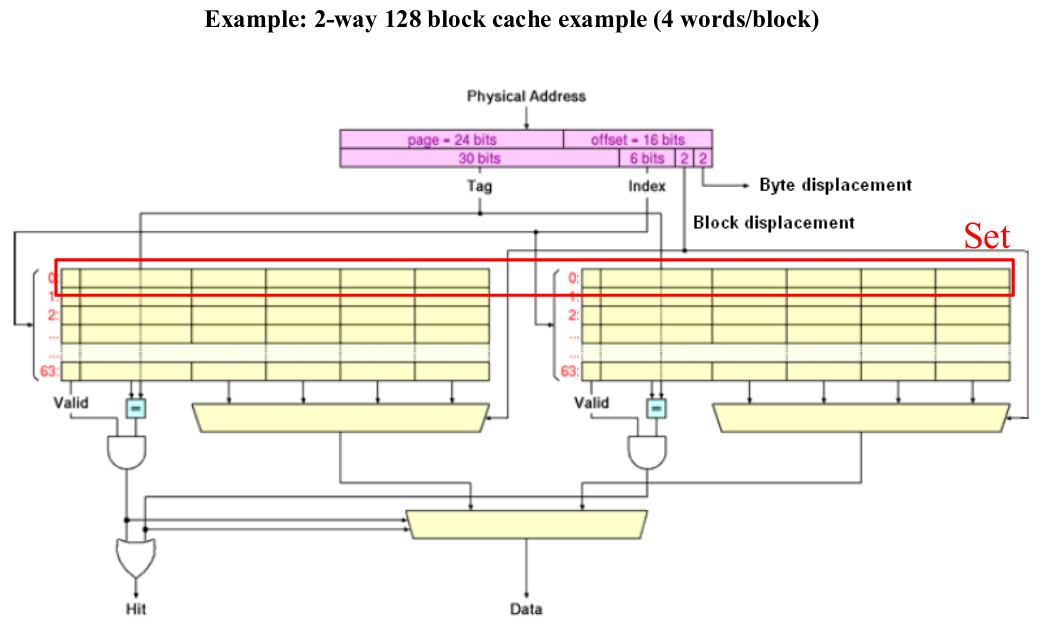
\includegraphics[width=\textwidth]{images/n-way_set_associative.png}

The direct mapped cache is a 1-way set associative cache (set = 1 block).
The fully associative cache has only one big set, the size of the whole cache.

\textbf{Advantages compared to fully associative cache}: comparators are fewer and smaller so cheaper and faster solutions.

\textbf{Advantages compared to direct-mapped cache}: better exploitation of temporal locality at a reasonable cost

The replacement of a block is performed by one of the techniques seen for associative cache (random, LRU or round-robin).

\section{Causes of cache miss}
\begin{itemize}
    \item \textbf{Compulsory misses}:\\
    at the time of the first access, a block is never present in cache. Not dependent on cache size and architecture (dependent on block size, though)
    \item \textbf{Capacity misses}:\\
    if the cache cannot contain all the blocks needed during execution of a program, capacity misses will occur due to blocks being discarded and later retrieved. This kind of misses decreases with cache size
    \item \textbf{Conflict misses}:\\
    in direct-mapped or set-associative caches, blocks that are replaced may have to be reloaded later in the same set – leading to collision (“conflict”) misses
\end{itemize}

\subsection{The write problem}
Write in caches are less frequent than reads.
Instruction fetch only requires memory reads.
“Load” instructions more frequent than “store”.

In Write to memory operations we ask:
\textbf{Speed}: implies writing to cache;
\textbf{Consistency}: information in lower-layer memories must always be consistent with information in cache.

\subsubsection{Write strategies:}
\paragraph{Write-through}
information is written \textbf{simultaneously} in cache block and in the main memory block. Consistency always respected, access time for writes is that of the lower level of memory, so lower performance.

\paragraph{Write-back}



\chapter{Branch Prediction}



\end{document}
